\chapter{Koncepcja powiązania analizy sentymentu i geolokacji w badaniu
zachowań użytkowników sieci społecznościowych.}
\label{chapter:koncepcjarozwiazania}

W tym rozdziale opisany jest sposób realizacji celów mojej pracy magisterskiej
-- czyli sposób powiązania ze sobą analizy sentymentu i geolokacji w kontekście
badania zachowań użytkowników sieci społecznościowych. W podrozdziale
\ref{section:modelsystemu} zaprezentowany został model systemu z uwzględnieniem
przetwarzania wstępnego w \ref{subsection:zbieraniedanych}, modelu analizy
sentymentu w \ref{subsection:modelanalizysentymentu}, modelu grup społecznych w
\ref{subsection:modelgrupirelacjispolecznych} i modelu geolokacji w
\ref{subsection:modelgeolokacji}. Następnie przedstawione są wielkości
wykorzystywane w eskperymentach w \ref{section:wielkosciwykorzystywane}, a na
końcu szczegółowo została opisana koncepcja i algorytm analizy sentymentu w
\ref{section:koncepcjaialgorytmanalizysentymentu}.



% =============================================================================
\section{Model systemu}
\label{section:modelsystemu}
% =============================================================================
Ogólny model systemu został przedstawiony na rysunku \ref{image:model-systemu}.

\begin{figure}[ht!]
\centering
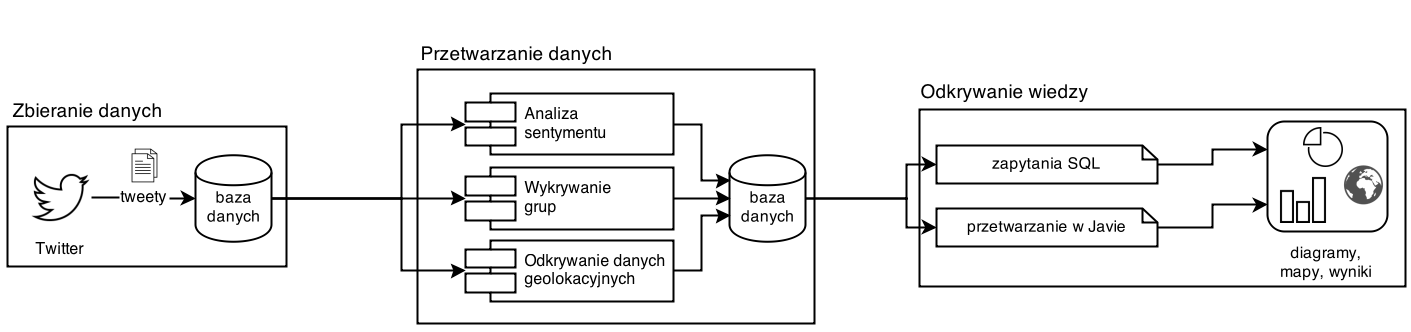
\includegraphics[width=160mm]{img/gruby-model.png}
\caption{Ogólny model systemu}
\label{image:model-systemu}
\end{figure}


Można go podzielić na trzy następujące części:
\begin{enumerate}
  \item Zbieranie danych.
  \item Przetwarzanie i uzupełnianie danych.
  \item Zdobywanie wiedzy z zebranych i przetworzonych danych.
\end{enumerate}



\clearpage
\subsection{Zbieranie danych}
\label{subsection:zbieraniedanych}
Zbieranie danych jest pierwszym elementem składowym całego systemu.
Jego koncepcje przedstawia rysunek \ref{image:zbieranie-danych}.
Jest to bardzo ważny składnik systemu. Aby móc przeprowadzić jakiekolwiek
analizy potrzeba najpierw zebrać dane.

\begin{figure}[ht!]
\centering
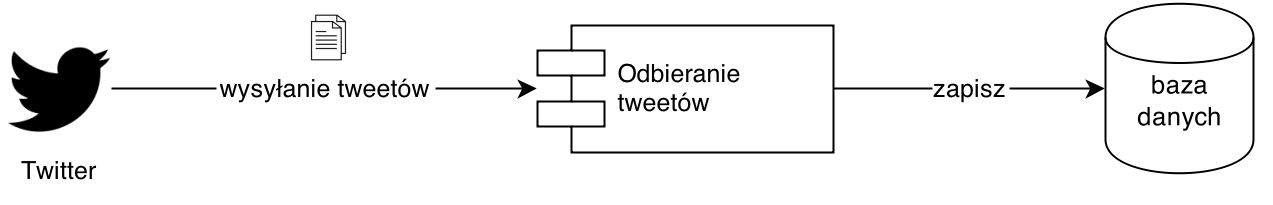
\includegraphics[width=160mm]{img/zbieranie-danych.png}
\caption{Zbieranie danych}
\label{image:zbieranie-danych}
\end{figure}


Zbieranie danych z serwisu Twitter odbyło się przy pomocy wspomnianego w sekcji
\ref{subsection:twitterjakozrodlodanych} Twitter Streaming API. Napisany został
program w Javie, który nasłuchiwał w trakcie każdego śledzonego meczu wpisów w
języku angielskim, które zawierały odpowiednie słowa kluczowe. Były nimi
przygotowane wcześniej słowa związane z danym spotkaniem: nazwiska i przydomki
piłkarzy, menadżerów, nazwy i przydomki klubów, nazwa stadionu czy nazwisko
sędziego. W taki sposób uzyskiwano tweety, które można było powiązać z
konkretnym meczem.

Program do nasłuchiwania uruchamiany jest na czas trwania meczu z pewnym
marginesem przed i po spotkaniu. Jest to o tyle ważne, że udostępnione API służy
tylko do konsumowania wpisów na żywo. Pobranie tych samych wpisów już po danym
wydarzeniu byłoby dużo bardziej skomplikowane. Program otrzymuje nie więcej niż
1\% wszystkich wpisów w danym momencie na Twitterze \footnote{Jeśli w danym
momencie na Twitterze jest 1000 wpisów, z czego 10 z podanymi słowami
kluczowymi, wówczas program otrzyma wszystkie 10 wpisów. Jeśli z określonymi
słowami kluczowymi byłoby np. 100 z 1000 wpisów, wówczas program nadal
otrzymałby tylko 10 z nich.}. Każdemu wpisowi nadawany jest identyfikator meczu (wprowadzonego
wcześniej do bazy danych) i w takiej postaci jest on zapisywany do bazy.

W ten sposób zbieranie są dane z Twittera. Podejście to pozwala na elastyczną
wymianę słów kluczowych do nasłuchiwania, gdyż program na wejściu potrzebuje
jedynie identyfikator meczu, do którego już są przypisane słowa kluczowe.




\subsection{Model analizy sentymentu}
\label{subsection:modelanalizysentymentu}

Analiza sentymentu należy do jednego z elementów drugiej części systemu.
W tej części zebrane uprzednio dane były przetwarzane między innymi pod kątem
oceny ich sentymentu. Proces ten przebiegał według schematu
zaprezentowanego na rysunku \ref{image:model-analizy-sentymentu}.

\begin{figure}[ht!]
\centering
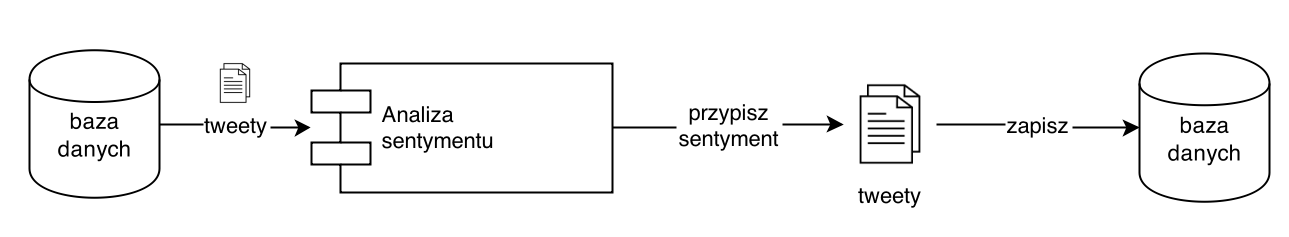
\includegraphics[width=160mm]{img/model-analizy-sentymentu.png}
\caption{Model analizy sentymentu}
\label{image:model-analizy-sentymentu}
\end{figure}


Dla każego tweeta w bazie obliczana była jego wartość \textit{valence}.
Aby do tego doszło tweet był wcześniej odpowiednio oczyszczany z wszystkich
elementów, które mogły zakłócić wyliczenie tej wartości. Proces przebiegał
zgodnie z pomysłem i algorytmem panów Pak i Paroubek (omówiony w sekcji
\ref{subsubsection:pakandparoubek}), a szczegóły jego działania wraz z
zastosowaną przez ze mnie modyfikacją (polegającą na dodaniu wykrywania negacji)
zostały opisane w sekcji \ref{section:koncepcjaialgorytmanalizysentymentu}.

Po wyliczeniu wartości \textit{valence} dla zebranych tweetów obliczona została
jego średnia wartość i wpisy o wartości wyższej od średniej zostały oznaczone
jako pozytywne, zaś o wartości niższej jako negatywne (zgodnie z pomysłem Paka
i Paroubeka).

Oznaczenie wartości sentymentu zebranych wpisów pozwoliło na przeprowadzenie
ciekawych eksperymentów opisanych w rozdziale \ref{chapter:eksperymenty}.


\subsection{Model grup i relacji społecznych}
\label{subsection:modelgrupirelacjispolecznych}
Drugim ważnym elementem przetwarzania zebranych danych było skupienie się na
odkrywaniu relacji między użytkownikami Twittera i odnajdywaniu grup, które
wspólnie tworzą. Pomaga to w lepszym zrozumieniu zachowań użytkowników i
możliwości osobnej analizy różnych grup. Schemat odkrywania zachowań społecznych
został przedstawiony na rysunku \ref{image:odkrywanie-relacji}.


\begin{figure}[ht!]
\centering
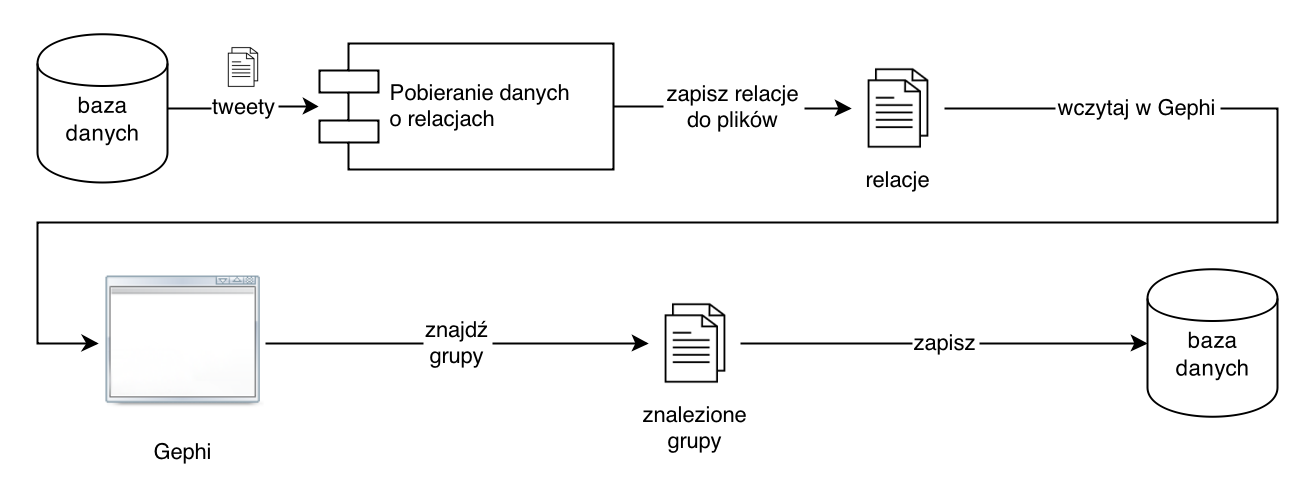
\includegraphics[width=160mm]{img/odkrywanie-relacji.png}
\caption{Model grup i relacji społecznych}
\label{image:odkrywanie-relacji}
\end{figure}


Sieć użytkowników zamodelowana jest w postaci grafu, gdzie użytkownicy to
wierzchołki, a wpisy będące retweetami lub odpowiedziami są krawędziami
(skierowanymi) tego grafu. Relacje te są przechowywane bezpośrednio w każdym z
tweetów w polach \texttt{in\_reply\_to\_user\_id} oraz
\texttt{retweeted\_user\_id}.
Do konkretnych eksperymentów dane te były odpowiednio agregowane (np. zliczano
liczbę powiązań między wierzchołkami i traktowano je jako pojedynczą relację w
jakiejś jednostce czasu -- na przykład w pojedynczym meczu).

Odkrywanie grup zostało przeprowadzone przy pomocy algorytmu opisanego w
\cite{FastUnfoldingOfCommunites}, który został zaimplementowany w środowisku
Gephi. Wyniki klasyfikacji wierzchołków do odpowiednich grup zostały następnie
zapisane w bazie danych.


\subsection{Model geolokacji}
\label{subsection:modelgeolokacji}
Ostatnim elementem przetwarzania zebranych danych było przetwarzanie związane z
danymi geolokacyjnymi. Przechowywane w bazie tweety posiadają jedynie współrzędne
określające miejsce, z którego zostały wysłane (oczywiście niewielki odsetek
tweetów z całego zbioru). Schemat przetwarzania tych danych prezentuje rysunek
\ref{image:odkrywanie-geolokacji}.

\begin{figure}[ht!]
\centering
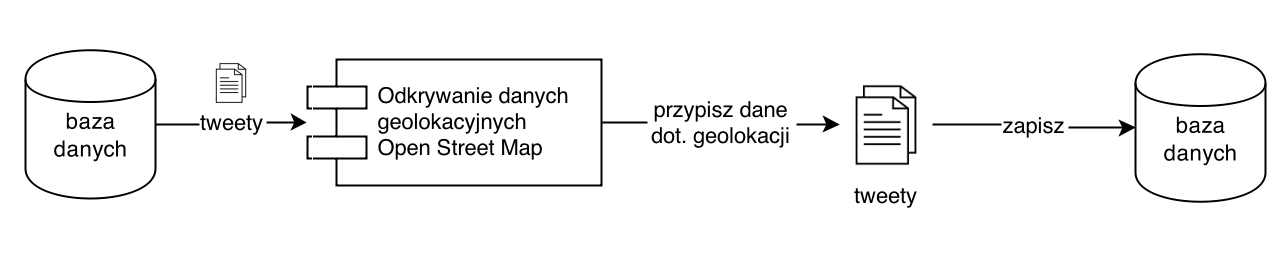
\includegraphics[width=160mm]{img/odkrywanie-geolokacji.png}
\caption{Model geolokacji}
\label{image:odkrywanie-geolokacji}
\end{figure}

Przy pomocy serwisu \textit{Open Street Map}\footnote{www.openstreetmap.com} i
skorzystaniu z API służącego do georeversingu dla każdego tweeta posiadającego
współrzędne pobrano informacje szczegółowe na temat miejsca, na które te
współrzędne wskazują. W ten sposób uzyskano takie dane jak: kraj,
stan/województwo (ang. \textit{state}), powiat/hrabstwo (ang. \textit{county})
oraz miasto (ang. \textit{city}).

Dodatkowo zaprezentowano w pracy mapy cieplne uwidaczniające częstość wpisów z
różnych lokalizacji na całym świecie. Do tego zadania skorzystano z usługi
\textit{CartoDB}\footnote{www.cartodb.com}, za pomocą której dostarczając dane
z geolokacją można otrzymać takiego rodzaju mapy.




% ==============================================================================
\section{Wielkości i techniki wykorzystywane w eksperymentach}
\label{section:wielkosciwykorzystywane}
% ==============================================================================
W tej sekcji zaprezentowane są wielkości i techniki, które zostały zastosowane w
zaprezentowanych w rozdziale \ref{chapter:eksperymenty} eksperymentach.
Przedstawione są one z podziałem na moduł, którego dotyczą.

\subsection{Analiza sentymentu}
Użyte w eksperymentach użyte miary i techniki związane z analizą sentymentu.

\subsubsection{Ocena pozytywności wpisów}
\label{subsection:ocenapozytywnosci}
Miara pozytywności wpisów określa ich sumaryczny wydźwięk. Jest to stosunek
liczby wpisów pozytywnych do sumy liczby wpisów pozytywnych i negatywnych. Gdy
wartość ta jest większa niż 50\% można mówić o wydźwięku pozytywnym, a gdy
mniejsza -- o negatywnym. Wartość tę określa się poniższym wzorem: 

\begin{equation}
\label{equation:pozytywnosc}
P = \frac{|pos|}{|pos| + |neg|}
\end{equation}

gdzie:

$|pos|$ -- liczba wpisów oznaczonych jako pozytywne,

$|neg|$ -- liczba wpisów oznaczonych jako negatywne.



\subsubsection{Wykrywanie zwolenników i przeciwników klubu}
\label{subsubsection:wykrywaniezwolennikow}

Dzięki oznaczeniu wszystkich zebranych wpisów odpowiednim sentymentem
(pozytwnym lub negatywnym) możliwe były wykorzystanie tych informacji do
odkrywania nowej wiedzy. Sentyment ten umożliwił odkrywanie wśród wszystkich
autorów wpisów ich preferencji klubowych -- poprzez zliczanie liczby wpisów
pozytywnych i negatywnych w meczach danego zespołu.

Proces oznaczania użytkowników jako sympatyków i przeciwników drużyny przebiegał
w następujący sposób:
\begin{itemize}
  \item dla każdego użytkownika zliczono jego wpisy w meczach każdej z badanych 
  drużyn,
  \item jeśli w meczach drużyny A dla danego użytkownika przeważała liczba 
  wpisów pozytywnych, wówczas oznaczano takiego kibica jako zwolennika drużyny A,
  \item jeśli natomiast przeważała liczba wpisów negatywnych, wówczas taki kibic
  traktowany był jako przeciwnik danej drużyny.  
\end{itemize} 

Zastosowanie tej techniki pozwala na przeprowadzenie eksperymentów z podziałem
na zwolenników i przeciwników danego klubu i zbadanie ich zachowań w zależności
od sympatii.




\subsection{Relacje między użytkownikami i grupy}
\label{subsection:miary-relacje}
W tej sekcji przedstawione zostały miary i techniki użyte podczas eksperymentów
związanych z odkrywaniem relacji i grup między użytkownikami.

\subsubsection{Wykrywanie grup}
\label{subsubsection:koncepcja-wykrywaniegrup}
% gephi, modularity
Do wykrywania grup wśród sieci społecznych zastosowałem model opisany w sekcji
\ref{subsection:modelgrupirelacjispolecznych}. Znalezione w ten sposób grupy
użytkowników poddane zostały analizie -- z podziałem na kolejne mecze.
Grupy te zostały zagregowane w trzy przedziały: od 3 do 4 osób, od 5 do 9 osób
oraz więcej niż 9 osób. Na takich zagregowanych grupach został przeprowadzony
eksperyment ich podobieństwa między kolejnymi meczami.

\subsubsection{Badanie podobieństwa grup}
\label{subsection:badaniepodobienstwagrup}
Tak jak wspomniano wyżej badanie podobieństwa oparte było o analizę kolejnych
wydarzeń (meczów).
Polegało na zliczeniu ile wierzchołków powtarza się w kolejnych spotkaniach.
Oparte zostało o poniższy wzór:
\begin{equation}
S = \frac{|V_1 \cap V_2|}{|V_1|}
\end{equation}  
gdzie:

$V_1$ -- zbiór wierzchołków w pierwszym wydarzeniu,

$V_2$ -- zbiór wierzchołków w następnym wydarzeniu.

Krótko mówiąc podobieństwo to iloraz liczby wspólnych wierzchołków między 
wydarzeniami a liczby wierzchołków w pierwszym z nich.







\subsection{Geolokacja}
W niniejszej sekcji opisuję wielkości, które zostały zastosowane podczas
przeprowadzania eksperymentów, w których najważniejszym elementem było położenie
fizyczne, czyli współrzędne przypisane do wpisu.

\subsubsection{Zmierzenie odległości między użytkownikami}
\label{subsubsection:zmierzenieodleglosci}


Badanie odległości między użytkownikami odbyło się na podstawie odpowiedzi z
geolokacją -- czyli tweetów zawierających dane o współrzędnych miejsca ich
wysłania oraz będących odpowiedziami (mającymi niepuste pole
\texttt{in\_reply\_to\_user\_id}). Wpisy typu retweet nie zawierają informacji
o położeniu użytkownika (taka informacja nie jest rejestrowana przez Twitter).

Zmierzenie odległości między użytkownikami odbyło się przy pomocy rozszerzenia
PostGIS\footnote{www.postgis.net} do bazy
PostgreSQL\footnote{www.postgresql.org}, z pomocą którego można obliczyć
odległość w metrach między dwoma punktami geograficznymi.

Cały proces przebiegał według następującego schematu:
\begin{itemize}
  \item pobierz wszystkie wpisy będące odpowiedziami (\textit{reply}) i
  zawierające współrzędne geograficzne,
  \item pogrupuj użytkowników w pary według tego, kto z kim się komunikował,
  \item wylicz średnie położenie każdego z użytkowników dla każdej konwersacji*,
  \item wylicz przy pomocy PostGIS-a odległość między nimi.
\end{itemize}

* średnie położenie użytkownika zostało wyliczone jako średnia arytmetyczna
długości i szerokości geograficznych jego wpisów w danej konwersacji.

Zmierzenie odległości między użytkownikami zostało użyte w eksperymencie
opisującym zależność odległości od częstości komunikacji.



\subsubsection{Badanie odległości kibiców od stadionu}
\label{subsubsection:badanieodleglosciodstadionu}
Do każdego nasłuchiwanego meczu zostały przypisane współrzędne miejsca, w którym
się odbywał -- czyli współrzędne stadionu gospodarza danego spotkania. Badanie
odległości kibiców od stadionu zostało przeprowadzone oddzielnie dla każdego meczu. Aby je
przeprowadzić zastosowano poniższy schemat działania:

\begin{itemize}
  \item pobierz wszystkie wpisy posiadające współrzędne geograficzne (a więc
  nie tylko te będące odpowiedziami, jak w powyższym badaniu),
  \item wylicz średnie położenie każdego użytkownika z podziałem na spotkania,
  \item wylicz przy pomocy PostGIS-a odległość użytkownika od stadionu.
\end{itemize}

Badanie zostało przeprowadzone z podziałem na zwolenników i przeciwników i
pokazuje zależność odległości kibiców od miejsca rozegrania meczu w zależności
czy ich ulubiona drużyna gra mecz u siebie czy na wyjeździe.










% ==============================================================================
\section{Koncepcja i algorytm analizy sentymentu}
\label{section:koncepcjaialgorytmanalizysentymentu}
% ==============================================================================

W tym miejscu opisuję dokładnie koncepcję wyznaczania wydźwięku wypowiedzi i
zastosowany algorytm do analizy sentymentu. Przedstawiam czynności wstępne jakie
zostały zastosowane na tekście, prezentuję wybrany algorytm i zastosowane
w nim modyfikacje oraz opisuję sposób aplikacji algorytmu na przykładowych
tweetach.

\subsection{Normalizacja tekstu}
\label{subsection:normalizacjatekstu}
% pozbycie się słów kluczowych, zaprzeczenia, retweety

W związku z tym, że wpisy są tworzone przez zwykłych użytkowników posiadają one
wiele znaków i elementów, które z punktu widzenia analizy sentymentu są zbędne,
a czasami prowadzące do błędów. Dlatego też tekst należy poddać normalizacji,
usunięciu zbędnych elementów, szumów i spamu. Przykładowe wpisy przed i po
normalizacji przedstawia tabela \ref{tab:wpisy-normalizacja}.


\begin{table}[ht!]  
\begin{center}  
\begin{tabular}{|r|p{70mm}|p{70mm}|}
\hline
 & Przed normalizacją & Po normalizacji
\\ \hline

1 
& RT @J\_SPEKZ: Haha quality! \#Fellaini \#United \#Moyes http://t.co/rJB4K1fvZy
& --

\\ \hline

2
& Stay woke brah! The Arsenal is about to make everything alright soon :) RT
@JCphoenixx: So damn tired, So not sleepy. 
& stay woke brah make alright

\\ \hline

3 
& @abdul1haseeb My arsenal is not disappointing too :P
& not\_disappointing
 
\\ \hline

4 
& @Arsenal didn't think i could respect @aaronramsey any more than i already
did, bute what a gentleman he is for not to celebrate that goal:) 
& didnt not\_respect bute gentleman not\_celebrate not\_goal

\\ \hline

5 
& OHHHHHH!!!!! SO CLOSE!!! Wilshere!!! Good Job Ramsey keeping that move alive
& ohhhhhh close good job keeping alive

\\ \hline

6 
& Haha, you gotta agree, no one gets booed like Manchester United :D \#ZeDevilza
& haha gotta agree not\_booed

\\ \hline
\end{tabular} 
\end{center} 
\caption{Wpisy przed i po normalizacji}
\label{tab:wpisy-normalizacja}
\end{table}

Kolejne kroki, które przekształciły tweety do takiej postaci to:
\begin{enumerate}
  \item Usunięcie skomentowanych retweetów.\\
  \texttt{Stay woke brah! The Arsenal is about to make everything
  alright soon :) \sout{RT @JCphoenixx: So damn tired, So not sleepy.}}
  
  \item Usunięcie skomentowanych cytowań. \\
  \texttt{At all...\sout{"@dotun\_somoye: Even city's first goal
  negredo was offside....:( the refs not helping at all"} }
  
  \item Usunięcie hiperlinków.\\
  \texttt{You up for Arsenal's match later on? - what time? maybe if i'm not
  busy baby sitting :) \sout{http://t.co/aC5Ec8ipy1}}
 
  
  \item Usunięcie nazw użytkowników.\\
  \texttt{\sout{@abdul1haseeb} My arsenal is not disappointing too :P}
  
  
  \item Usunięcie hashtagów. \\
  \texttt{Haha, you gotta agree, no one gets booed like Manchester United :D
  \sout{\#ZeDevilza}}
  
  
  \item Oznaczenie wyrazów zaprzeczonych przedrostkiem \texttt{NOT\_} (opisuję
  dokładniej w sekcji \ref{subsection:sentyment-algorytm}). \\
  \texttt{didn't \textbf{NOT\_think NOT\_i NOT\_could NOT\_respect NOT\_any 
  NOT\_more NOT\_than NOT\_i NOT\_already NOT\_did}, bute what a gentleman he 
  is for not \textbf{NOT\_to NOT\_celebrate NOT\_that NOT\_goal:)}}

 \item Zachowanie tylko znaków alfabetu:
  	\begin{itemize}
  		\item usunięcie zaimków dzierżawczych (\texttt{Helen's} $\to$ \texttt{Helen}),
  		\item usunięcie apostrofu ze skróconych zaprzeczeń (\texttt{don't} $\to$ \texttt{dont}),
  		\item normalizacja liter diakrytyzowanych (\texttt{José Mourinho} $\to$ \texttt{Jose
  		Mourinho})
  		\item usunięcie liczb i wszelkich znaków niealfabetycznych.
	\end{itemize}

  \texttt{You up for Arsenal\sout{'s} match later on\sout{? -} what
  time\sout{?} maybe if i\sout{'}m not busy baby sitting \sout{:)}} 
	
	\item Usunięcie wyrazów zdefiniowanych w stop liście (powszechne wyrazy danego
	języka, które mogą być pominięte nie tracąc jednocześnie żadnej informacji).
	Zastosowałem stop listę z serwisu \mbox{WebPageAnalyse.com} 
	\cite{WebPageAnalyse} zawierającą 528 słów.

	\texttt{\sout{You up for} Arsenal match \sout{later on what} time \sout{maybe if} 
 	im \sout{not} busy baby sitting}
	
	\item Usunięcie słów kluczowych, które użyte były do gromadzenia wpisów z
	Twittera -- czyli nazwisk piłkarzy, menadżerów, nazw klubów, itd.
	
	%\texttt{\sout{BENDTNER} FUCKING im \sout{NOT\_arsenal} NOT\_fan}
	
	\texttt{OHHHHHH CLOSE \sout{Wilshere} Good Job \sout{Ramsey} keeping alive}
	
\end{enumerate}





\subsection{Zastosowanie algorytmu}
\label{subsection:sentyment-algorytm}
% + dobór parametrów, emotikony, zaprzeczenia

Do przeprowadzenia analizy sentymentu na zebranych tweetach skorzystałem z
metody opracowanej przez Alexandra Paka i Patricka Paroubek'a, którą 
przedstawiłem w sekcji \ref{subsubsection:pakandparoubek}.
Jest to technika, która pozwala badać sentyment nie posiadając wcześniej
słownika sentymentu. Dlatego też pierwszym krokiem jest zbudowanie takiego
słownika z zebranych danych.
W tym celu wybiera się podzbiór wpisów, które zawierają emotikony.
W związku ze 140-znakowym ograniczeniem na długość znaków przyjmuje się
założenie, że dana emotikona nadaje wydźwięk całemu wpisowi.

Według artykułu \cite{EmoticonAnalysisTwitter} 20 emotikon pokrywa w 90\%
stosowanie tych znaków graficznych we wpisach (na 100 wpisów z emotikonami, 90 z
nich zawiera emotikonę ze zbioru tych 20) na Twitterze. Dlatego też skorzystałem
z tego zbioru do własnych badań dzieląc emotikony na wyrażające wydźwięk pozytywny i
negatywny w sposób\footnote{emotikona \texttt{D:} została pominięta, gdyż
pokrywała więcej przypadków niż tylko użycie emotikony (np.:
\texttt{Accepte\textbf{d:} Mary, John, Jane})} przedstawiony w tabeli
\ref{tab:wydzwiek-emotikon}.

\begin{table}[ht!]  
\begin{center}  
\begin{tabular}{|c|r|l|}
\hline
Emotikona & Popularność (wg \cite{EmoticonAnalysisTwitter}) &
Wydźwięk \\ \hline
\texttt{:)} & $33.4\%$ & pozytywny \\ \hline
\texttt{:D} & $11.0\%$ & pozytywny \\ \hline
\texttt{:(} & $7.9\%$ & negatywny \\ \hline
\texttt{;)} & $7.5\%$ & pozytywny \\ \hline
\texttt{:-)} & $4.4\%$ & pozytywny \\ \hline
\texttt{:P} & $3.7\%$ & pozytywny \\ \hline
\texttt{=)} & $3.7\%$ & pozytywny \\ \hline
\texttt{(:} & $2.8\%$ & pozytywny \\ \hline
\texttt{;-)} & $2.2\%$ & pozytywny \\ \hline
\texttt{:/} & $1.9\%$ & negatywny \\ \hline
\texttt{XD} & $1.9\%$ & pozytywny \\ \hline
\texttt{=D} & $1.5\%$ & pozytywny \\ \hline
\texttt{:O} & $1.1\%$ & pozytywny \\ \hline
\texttt{=]} & $1.1\%$ & pozytywny \\ \hline
\texttt{;D} & $1.0\%$ & pozytywny \\ \hline
\texttt{:]} & $1.0\%$ & pozytywny \\ \hline
\texttt{:-(} & $0.8\%$ & negatywny \\ \hline
\texttt{=/} & $0.8\%$ & negatywny \\ \hline
\texttt{=(} & $0.8\%$ & negatywny \\ \hline
\end{tabular} 
\end{center} 
\caption{Wydźwięk emotikon}
\label{tab:wydzwiek-emotikon}
\end{table}

Następnie przeglądnięto wszystkie tweety z emotikonami zliczając liczbę
występowania wyrazów w kontekście pozytywnym i negatywnym.
Najpierw badano sentyment całego wpisu (na podstawie emotikony -- gdy była ich
większa ilość wybierano ten sentyment, który przeważał) a następnie dla każdego
wyrazu z tego wpisu zwiększano licznik odpowiednio wystąpień pozytywnych lub
negatywnych. Oczywiście wpisy były już poddane normalizacji.
W ten sposób uzyskano słownik sentymentu zbudowany z zebranych danych, który
zawierał 34183 słowa, a najpopularniejsze z nich zaprezentowane są w tabeli
\ref{tab:liczebnosc-slow-sentymentu}, gdzie:

wartość \textit{valence} wyliczna jest według wzoru \ref{equation:pakparoubek} 
i używana jest w dalszych obliczeniach,

wartość pozytywności wyliczona jest według wzoru \ref{equation:pozytywnosc}.

\begin{table}[ht!]  
\begin{center}  
\begin{tabular}{|l|r|r|r|r|}
\hline
Słowo & Wyst. pozytywne  & Wyst. negatywne 
& Pozytywność
& Valence
\\ \hline 
win & 4206 & 598 & 87.6 \% & 0.845 \\ \hline
good & 3916 & 435 & 90.0 \% & 0.903 \\ \hline
game & 3016 & 1012 & 74.9 \% & 0.301 \\ \hline
goal & 2305 & 584 & 79.8 \% & 0.477 \\ \hline
today & 2019 & 526 & 79.3 \% & 0.477 \\ \hline
time & 1844 & 404 & 82.0 \% & 0.602 \\ \hline
dont & 1461 & 775 & 65.3 \% & 0.000 \\ \hline
match & 1669 & 449 & 78.8 \% & 0.477 \\ \hline
great & 1885 & 160 & 92.2 \% & 1.041 \\ \hline
love & 1837 & 202 & 90.1 \% & 0.954 \\ \hline
\end{tabular} 
\end{center} 
\caption{Liczba występowania najpopularniejszych słów w zbudowanych słowniku
sentymentu}
\label{tab:liczebnosc-slow-sentymentu}
\end{table}

Dla każdego wpisu wyliczana jest średnia arytmetyczna wartości \textit{valence}
wszystkich słów. W ten sposób wylicza sie wartość \textit{valence} danego wpisu.
W tabeli \ref{tab:valence-przyklad} prezentuję przykładowe wyniki wyliczania tej
wielkości.

\begin{table}[ht!]
\begin{center}  
\begin{tabular}{|p{12mm}|p{70mm}|>{\raggedright\arraybackslash}p{60mm}|}
\hline
Valence & Wpis & Składowe 
\\ \hline 
0.6261 POS & Just seen you in the crowd at Chelsea game! @domashman http://t.co/NjovoZdgZ3 & {game=0.4740, crowd=0.7782}
\\ \hline
0.5909 POS & RT @BTSP: \#PRIZEDRAW If Arsenal win tonight one lucky person
will win a personalised BTSP mug! Simply RT \& follow to enter!
http://t.co/9m... & {lucky=0.4613, tonight=0.6873, btsp=0.3010, person=0.4232, personalised=0.3010, enter=0.5351, follow=1.2229, win=0.8465, mug=0.4771, simply=0.3979}
\\ \hline
0.6199 POS & Liking the brightness of this Napoli kit \#tempted &
{liking=0.8062, kit=0.4337} \\ \hline
0.0305 NEG & @ricktaylor1987 You're not watching Arsenal? &
{not\_watching=0.0305} \\ \hline
0.1234 NEG & Poor start\#AFC & {poor=-0.2848, start=0.5317}
\\ \hline
0.1807 NEG & Do Arsenal have any players who don't fall down with ease?
\#SwimmingTeam & {players=0.3684, not\_fall=-0.3979, not\_ease=0.4771,
dont=0.2751} \\ \hline
\end{tabular} 
\end{center} 
\caption{Wynik działania algorytmu analizy sentymentu na przykładowych wpisach}
\label{tab:valence-przyklad}
\end{table}

Określenie sentymentu wpisu odbywa się zgodnie z równaniem:
\begin{equation}
S(t) =
\begin{cases}
POS & valence(t) > AVG\_VALENCE \\
NEG & valence(t) <= AVG\_VALENCE \\
\end{cases}
\end{equation}

gdzie:

$AVG\_VALENCE$ jest średnią arytmetyczną wartości $valence$ wszystkich wpisów.
%wszystkich wpisów. W moich badaniach wartość ta wyniosła $0.4786984978198536$.

\subsection{Wykrywanie i obsługa negacji}
\label{subsubsection:wykrywanieiobsluganegacji}
W oryginalnym podejściu panów Pak i Paroubek nie ma żadnego sposobu na
wykrywanie i obsługę negacji. Oczywistym jednak jest, iż zaprzeczenia zmieniają
znaczenie dalszej części tekstu i muszą być w jakiś sposób obsłużone.
Wpisy na Twitterze są krótkie, więc postanowiłem zastosować podejście
zaprezentowane w artykule \cite{thumbsUp2002}, które polega na dodaniu
przedrostka \texttt{NOT\_} do wszystkich słów pomiędzy wyrazem negującym
a najbliższym znakiem przestankowym. Lista wyrazów negujących
została zaczerpnięta z \cite{englishNots1983}. Słowa zanegowane miały osobno
liczone liczby wystąpień w kontekstach pozytwnych i negatywnych. W takiej formie
brały udział w ocenie sentymentu wpisów z Twittera.







\subsubsection{Dobór parametrów}
\label{subsubsection:doborparametrow}
Użyty przeze mnie algorytm zakłada dobór parametrów przed przeprowadzeniem
analizy sentymentu. Parametry te dotyczą słów ze zbudowanego słownika --
decydując, które z nich wezmą udział w procesie analizy. Są to: minimalna
długość słowa, minimalna liczba występowania słowa. Doboru parametrów dokonałem
w sposób zaprezentowany w opisie algorytmu. Wykorzystałem listę wpisów z
emotikonami, podzieliłem je na zbiór uczący i testowy w stosunku 20\% do 80\%.
Wygenerowałem słownik ze zbioru uczącego. Wpisy ze zbioru testowego oznaczyłem spodziewanym
sentymentem -- był to sentyment emotikony jaką zawierały. Następnie
przeprowadziłem testy poprawności klasyifkacji zbioru testowego słowami ze
zbioru uczącego dla wyrazów o minimalnej długości od 1 do 10 i minimalnej
liczbie wystąpień od 1 do 100 -- daje to w sumie 1000 testów.
Najwyższy stopień poprawności klasyfikacji uzyskałem dla parametrów równych:
minimalna długość wyrazu -- 3, \mbox{minimalna częstotliwość wystąpień -- 1}.
Wyniki testów przedstawiam na wykresie
\ref{image:pak-paroubek-parametry}.

\begin{figure}[ht!]
\centering
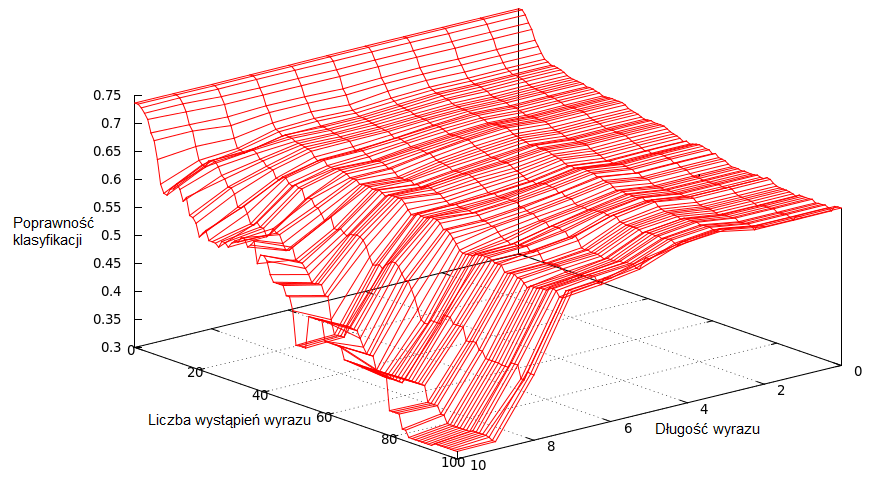
\includegraphics[width=160mm]{img/pak-paroubek-params_pl.png}
\caption{Dobór parametrów algorytmu analizy sentymentu}
\label{image:pak-paroubek-parametry}
\end{figure}